\section{Results}
\label{sec:results}

\subsection{Main Comparison Against Classical Baselines}

\begin{table}[t]
    \centering
    \resizebox{\textwidth}{!}{%
    \begin{tabular}{@{}lcccc@{}}
        \toprule
        \textbf{Method} & \textbf{MRR} & \textbf{NDCG@10} & \textbf{Hit@10} & \textbf{Mean Top-10 Popularity Pct} \\
        \midrule
        Popularity & 0.051 & 0.000 & 0.000 & 0.0001 \\
        Cooccurrence & 0.282 & 0.246 & 0.260 & 0.0100 \\
        \gptfourone (\minimalprompt) & {\bf 0.589} & {\bf 0.621} & {\bf 0.780} & 0.0388 \\
        \gptfourone (\profileprompt) & 0.539 & 0.581 & {\bf 0.780} & {\bf 0.0398} \\
        \claudesonnet (\minimalprompt) & 0.572 & 0.597 & 0.740 & 0.0361 \\
        \claudesonnet (\profileprompt) & 0.544 & 0.586 & {\bf 0.780} & 0.0397 \\
        \bottomrule
    \end{tabular}
    }
    \caption{Results on \lastfm next-track ranking. Higher is better for all metrics shown. Best results are in \textbf{bold}.}
    \label{tab:lastfm-results}
\end{table}

\begin{table}[t]
    \centering
    \resizebox{\textwidth}{!}{%
    \begin{tabular}{@{}lcccc@{}}
        \toprule
        \textbf{Method} & \textbf{MRR} & \textbf{NDCG@10} & \textbf{Hit@10} & \textbf{Mean Top-10 Popularity Pct} \\
        \midrule
        Popularity & 0.067 & 0.036 & 0.100 & 0.0012 \\
        Cooccurrence & 0.094 & 0.061 & 0.120 & 0.0494 \\
        \gptfourone (\minimalprompt) & {\bf 0.329} & {\bf 0.379} & 0.640 & {\bf 0.0832} \\
        \gptfourone (\profileprompt) & 0.203 & 0.206 & 0.380 & 0.0710 \\
        \claudesonnet (\minimalprompt) & 0.312 & 0.373 & {\bf 0.660} & 0.0805 \\
        \claudesonnet (\profileprompt) & 0.244 & 0.285 & 0.540 & 0.0747 \\
        \bottomrule
    \end{tabular}
    }
    \caption{Results on \mpd playlist continuation. Higher is better for all metrics shown. Best results are in \textbf{bold}.}
    \label{tab:mpd-results}
\end{table}


\para{\lastfm.} Table~\ref{tab:lastfm-results} shows that every LLM condition outperforms both classical baselines. The best configuration is \gptfourone with the \minimalprompt prompt, which reaches 0.589 \mrr and 0.621 \ndcg. This is a large absolute gain over \coocbaseline at 0.282 \mrr and 0.246 \ndcg. The bootstrap 95\% confidence interval for \gptfourone (\minimalprompt) is [0.464, 0.711] for \mrr and [0.508, 0.732] for \ndcg, while \coocbaseline reaches [0.171, 0.396] and [0.140, 0.366].

\para{\mpd.} Table~\ref{tab:mpd-results} shows the same pattern on playlist continuation. \gptfourone (\minimalprompt) reaches 0.329 \mrr and 0.379 \ndcg, compared with 0.094 and 0.061 for \coocbaseline. The corresponding bootstrap 95\% confidence intervals are [0.235, 0.434] and [0.277, 0.485] for \gptfourone (\minimalprompt), versus [0.061, 0.142] and [0.016, 0.119] for \coocbaseline.

\begin{figure}[t]
    \centering
    \begin{minipage}[t]{0.49\linewidth}
        \centering
        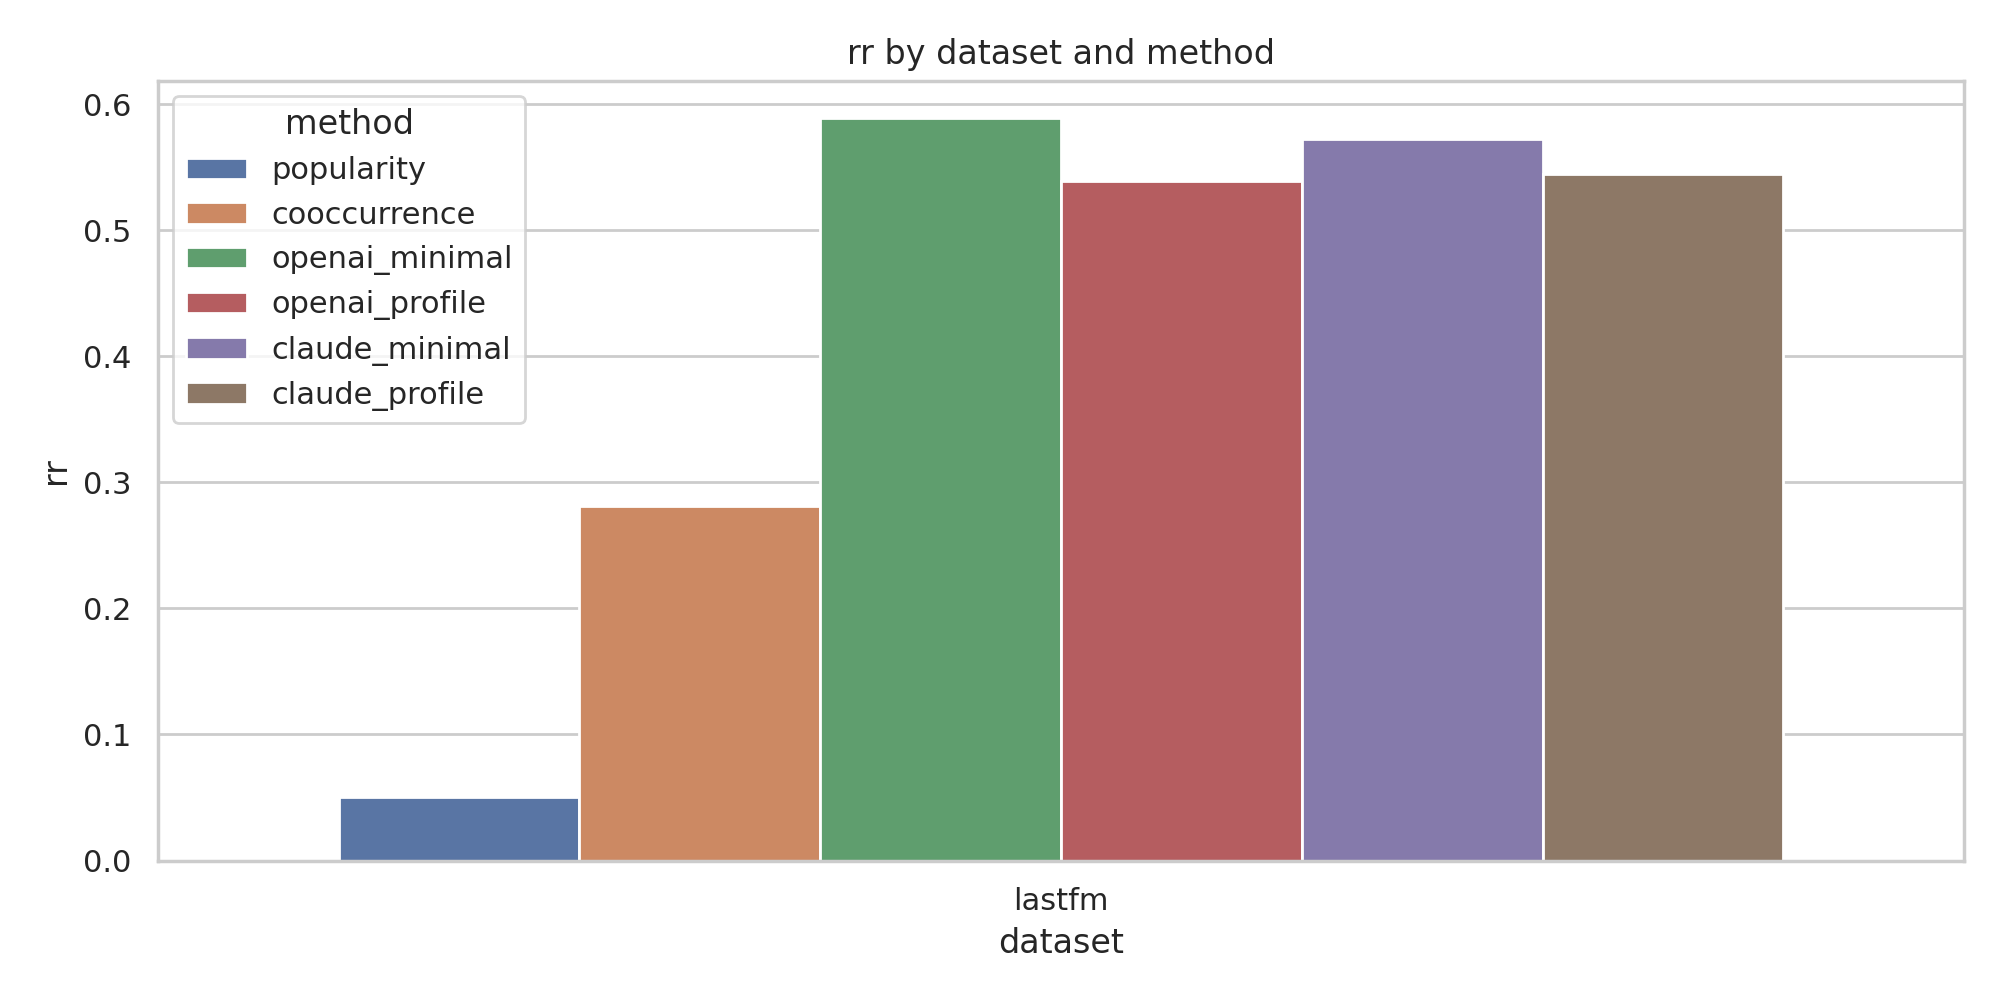
\includegraphics[width=0.95\linewidth]{figures/lastfm/rr_comparison.png}\\
        \vspace{2pt}
        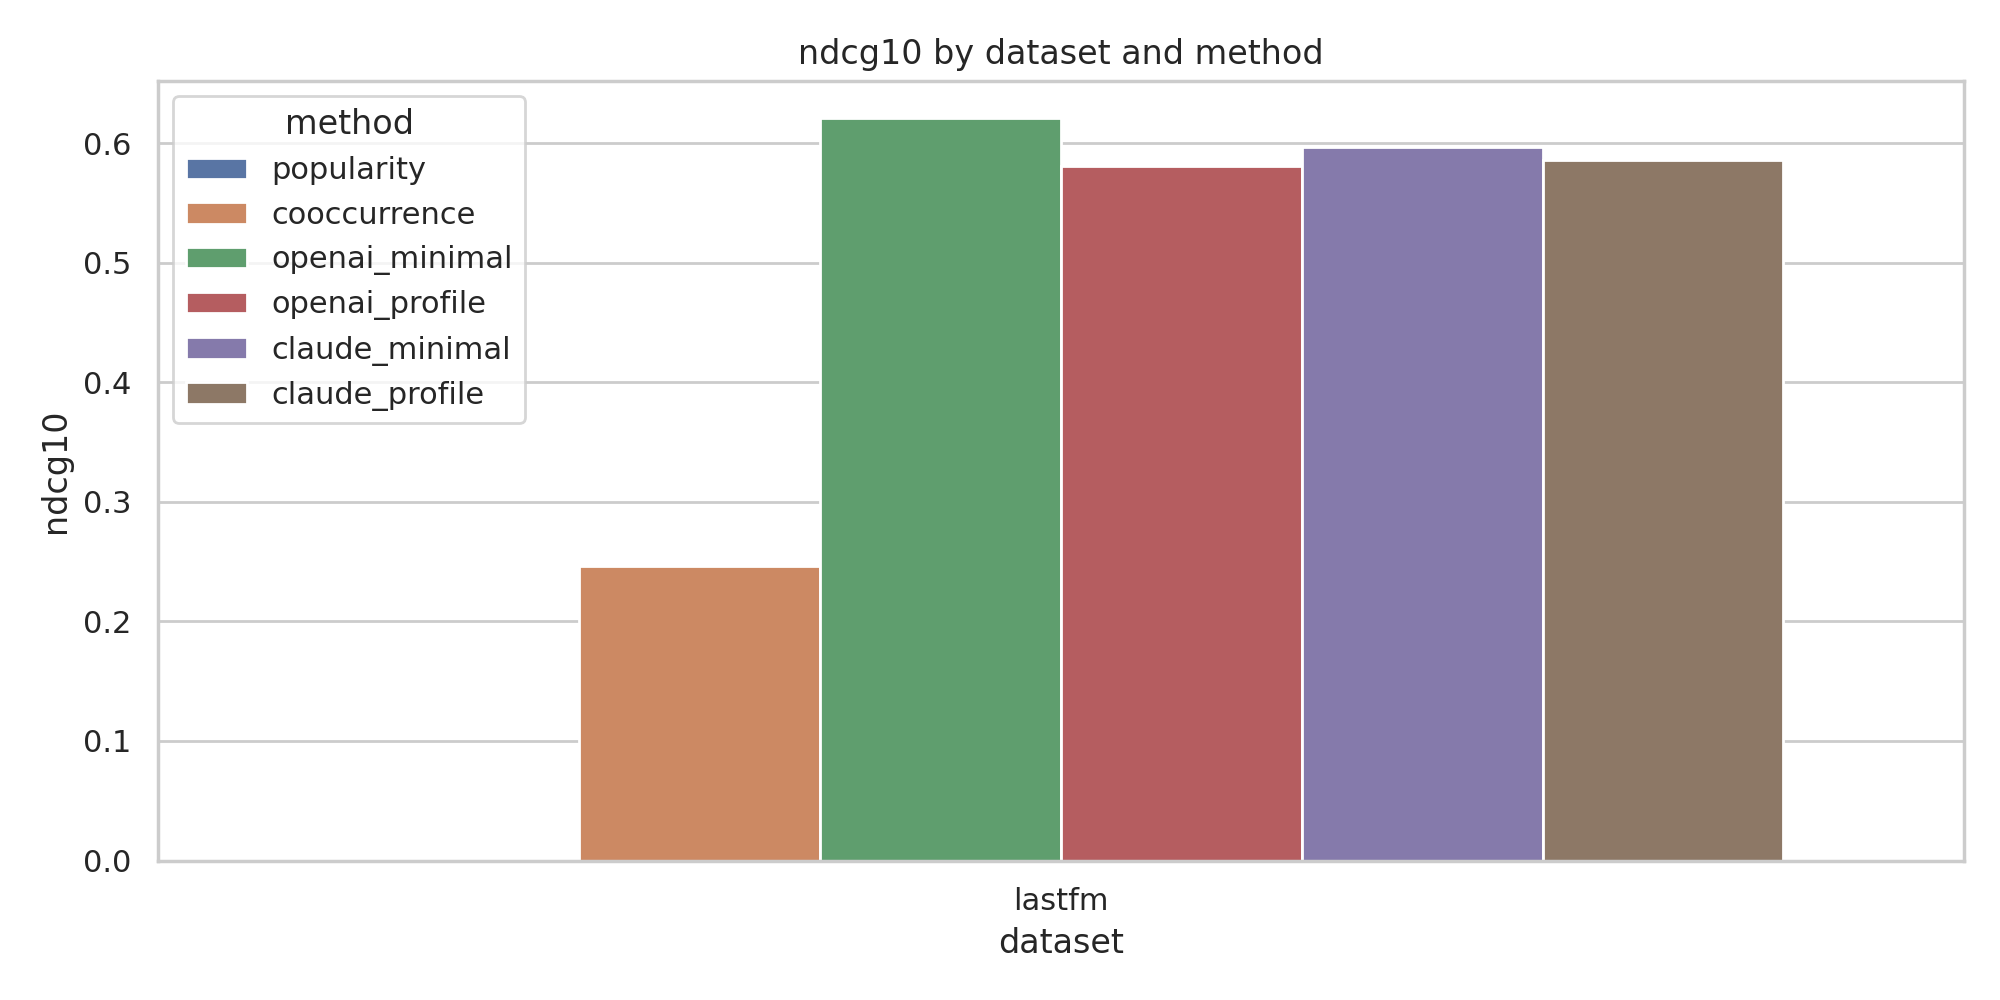
\includegraphics[width=0.95\linewidth]{figures/lastfm/ndcg10_comparison.png}
    \end{minipage}
    \hfill
    \begin{minipage}[t]{0.49\linewidth}
        \centering
        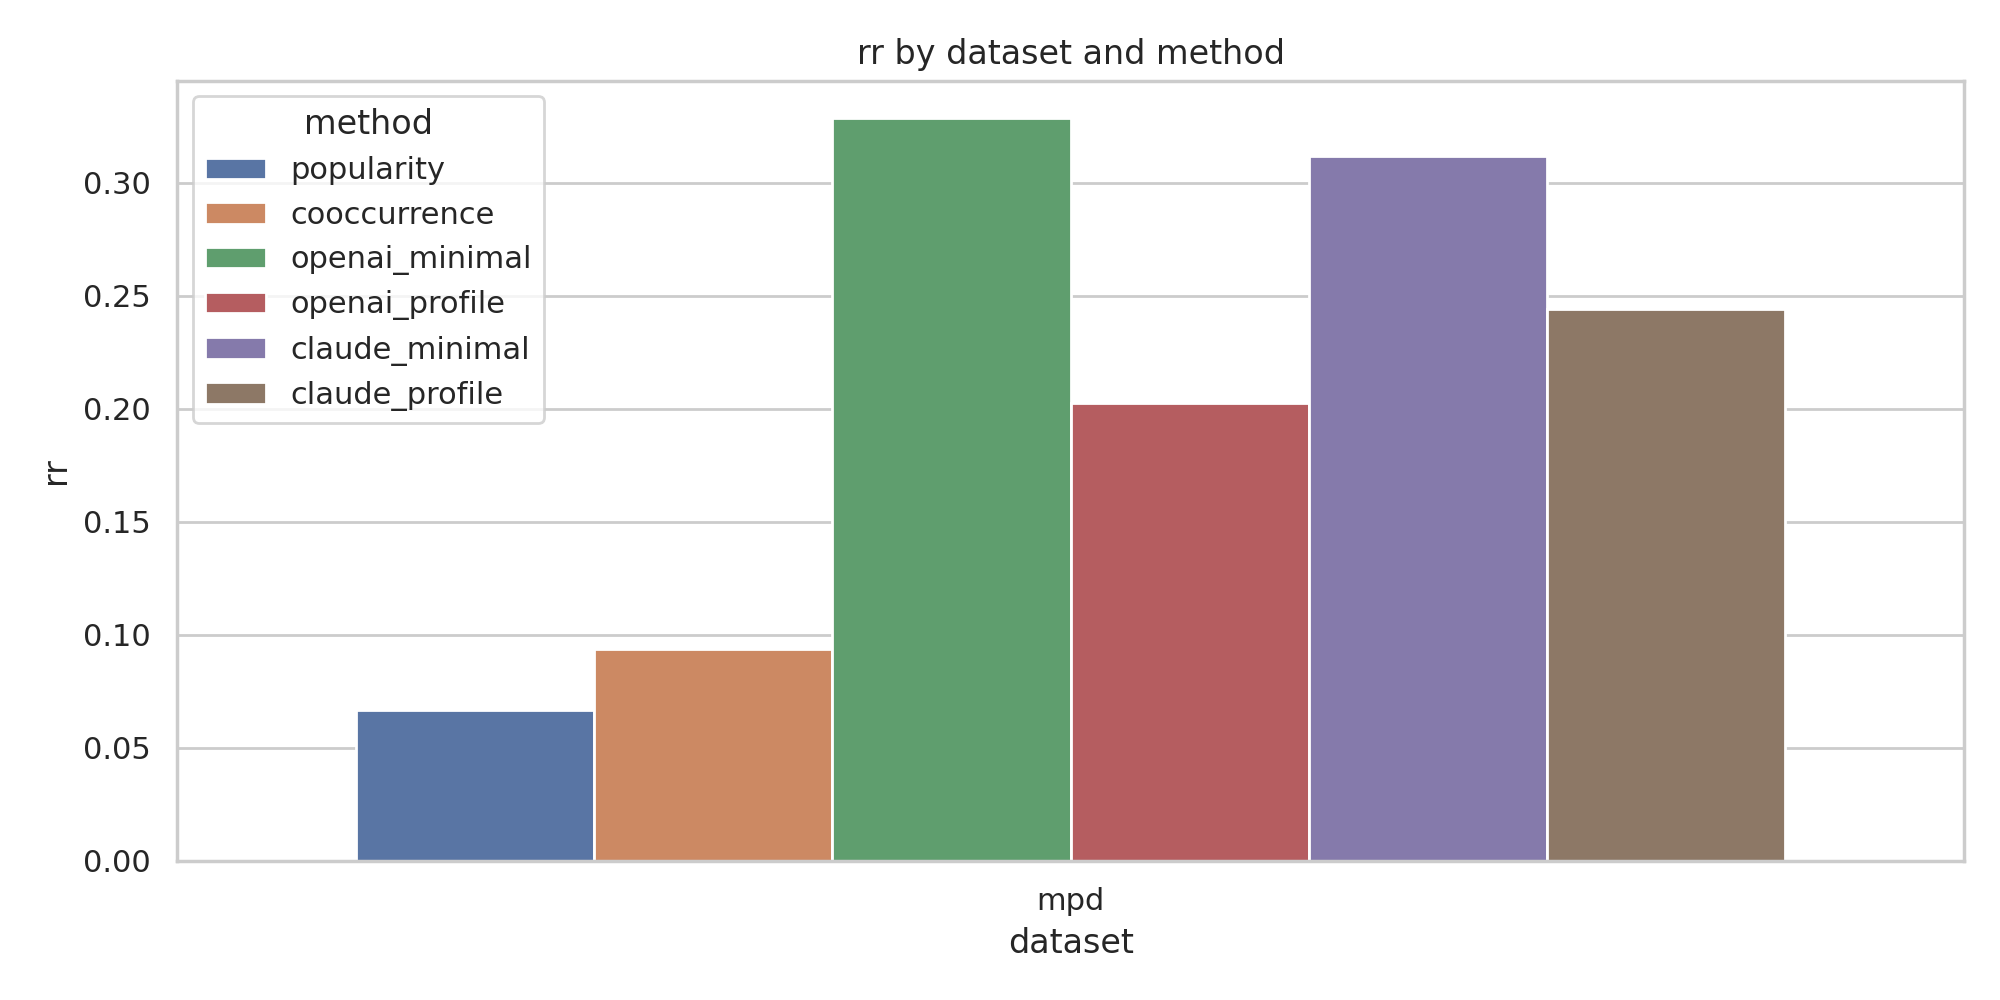
\includegraphics[width=0.95\linewidth]{figures/mpd/rr_comparison.png}\\
        \vspace{2pt}
        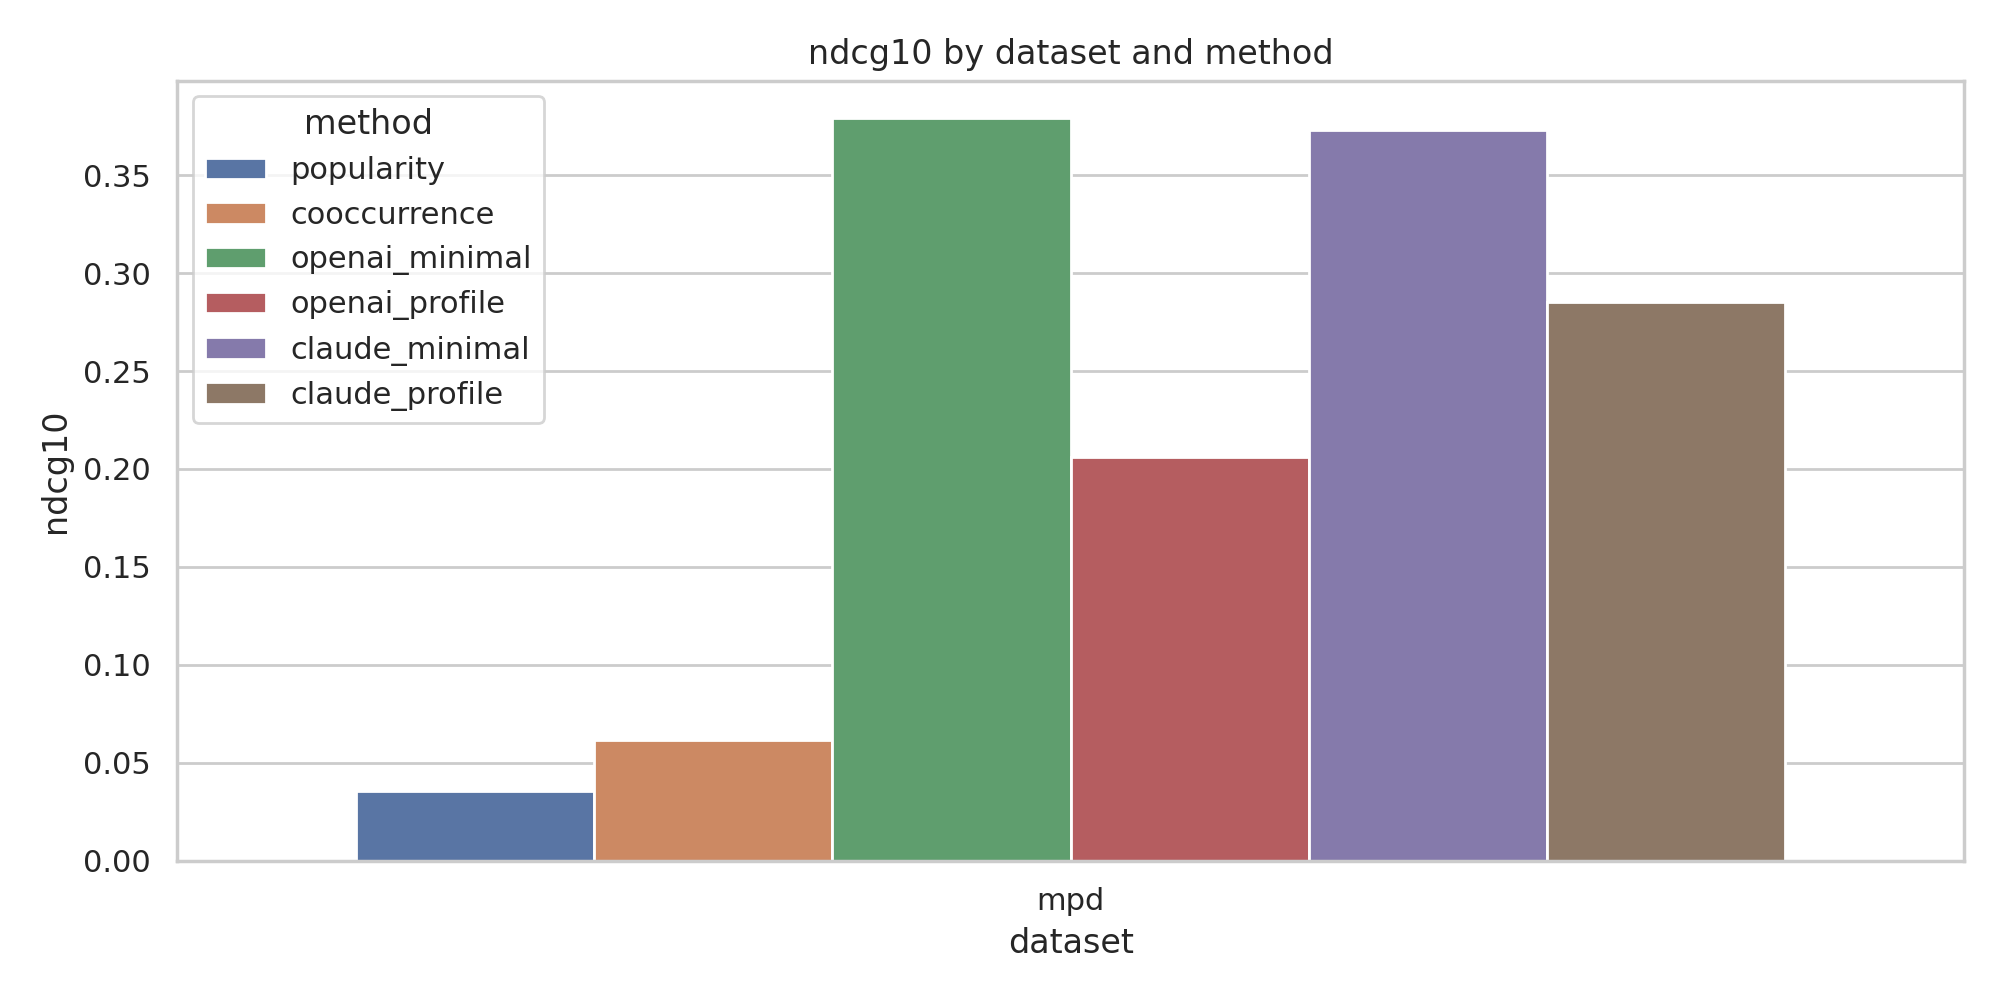
\includegraphics[width=0.95\linewidth]{figures/mpd/ndcg10_comparison.png}
    \end{minipage}
    \caption{Ranking performance on both datasets. Left column: \lastfm reciprocal rank and \ndcg comparisons. Right column: \mpd reciprocal rank and \ndcg comparisons. In both datasets, prompt-only LLM conditions separate clearly from the classical baselines, with the simplest prompt producing the strongest results.}
    \label{fig:main-results}
\end{figure}

\subsection{Significance Tests}

\para{Primary comparisons.} The gains over the strongest classical baseline remain significant after Benjamini-Hochberg correction on both datasets. On \lastfm, \gptfourone (\minimalprompt) beats \coocbaseline with corrected $p=4.69\times10^{-6}$ on \mrr and $p=1.44\times10^{-5}$ on \ndcg, with paired effect sizes $d=0.70$ and $d=0.85$. \claudesonnet (\minimalprompt) also beats \coocbaseline with corrected $p=1.10\times10^{-5}$ on \mrr and $p=3.82\times10^{-5}$ on \ndcg, with $d=0.62$ and $d=0.75$.

On \mpd, \gptfourone (\minimalprompt) beats \coocbaseline with corrected $p=3.57\times10^{-7}$ on \mrr and $p=7.88\times10^{-6}$ on \ndcg, with $d=0.69$ and $d=0.85$. \claudesonnet (\minimalprompt) shows similarly strong gains, with corrected $p=3.57\times10^{-7}$ on \mrr and $p=5.93\times10^{-6}$ on \ndcg, and effect sizes $d=0.72$ and $d=0.93$.

\subsection{Prompt Ablation and Model Comparison}

\para{Minimal prompts are enough.} The richer \profileprompt prompt does not improve performance. On \lastfm, the difference between \minimalprompt and \profileprompt is not significant for either model. On \mpd, the profile prompt is reliably worse. For \claudesonnet, \minimalprompt beats \profileprompt with $p=0.00138$ on \mrr and $p=0.00990$ on \ndcg. For \gptfourone, \minimalprompt beats \profileprompt with $p=0.00034$ on \mrr, $p=0.00114$ on \ndcg, and $p=0.00079$ on \hitten.

\para{Model comparison.} The best \gptfourone and \claudesonnet prompt-only systems are statistically tied on both datasets. On \mpd, for example, \gptfourone (\minimalprompt) and \claudesonnet (\minimalprompt) differ only by $p=0.963$ on \mrr and $p=0.891$ on \ndcg.

\subsection{Beyond-Accuracy Behavior}

\para{Popularity concentration.} The LLM conditions consistently achieve higher mean top-10 popularity percentiles than the classical baselines. On \lastfm, \gptfourone (\minimalprompt) reaches 0.0388 versus 0.0100 for \coocbaseline. On \mpd, the same comparison is 0.0832 versus 0.0494. Under this metric, larger values mean recommendations are less concentrated in the global popularity head.

\para{Coverage.} Coverage also increases modestly. On \lastfm, coverage rises from 0.00166 for \coocbaseline to 0.00175--0.00198 for the LLM conditions. On \mpd, coverage rises from 0.00988 for \coocbaseline to 0.01053--0.01194 for the LLM conditions. These gains are small in absolute value, but they indicate that accuracy improvements are not driven only by repeating the most common items.
